\documentclass{beamer}

\graphicspath{{./images/}}

\usetheme{Berlin}
\title{{\tt OOPS}: An $S5_n$ Prover for Educational Settings}
\author{Gert van Valkenhoef \and Elske van der Vaart \and Rineke Verbrugge}
\date{12 October, 2009}

\logo{
\includegraphics[height=0.5cm]{RUGR_logoEN_rood_RGB}}

\usepackage{listings}
% -*- latex -*-
% Definition of the Lua language for the listings package
% Time-stamp: <2008-11-30 15:27:16 rsmith>
% Written by Roland Smith <rsmith@xs4all.nl> and hereby placed in the public
% domain. 

\lstdefinelanguage{lua}
  {morekeywords={and,break,do,else,elseif,end,false,for,function,if,in,local,
     nil,not,or,repeat,return,then,true,until,while},
   morekeywords={[2]arg,assert,collectgarbage,dofile,error,_G,getfenv,
     getmetatable,ipairs,load,loadfile,loadstring,next,pairs,pcall,print,
     rawequal,rawget,rawset,select,setfenv,setmetatable,tonumber,tostring,
     type,unpack,_VERSION,xpcall},
   morekeywords={[2]coroutine.create,coroutine.resume,coroutine.running,
     coroutine.status,coroutine.wrap,coroutine.yield},
   morekeywords={[2]module,require,package.cpath,package.load,package.loaded,
     package.loaders,package.loadlib,package.path,package.preload,
     package.seeall},
   morekeywords={[2]string.byte,string.char,string.dump,string.find,
     string.format,string.gmatch,string.gsub,string.len,string.lower,
     string.match,string.rep,string.reverse,string.sub,string.upper},
   morekeywords={[2]table.concat,table.insert,table.maxn,table.remove,
   table.sort},
   morekeywords={[2]math.abs,math.acos,math.asin,math.atan,math.atan2,
     math.ceil,math.cos,math.cosh,math.deg,math.exp,math.floor,math.fmod,
     math.frexp,math.huge,math.ldexp,math.log,math.log10,math.max,math.min,
     math.modf,math.pi,math.pow,math.rad,math.random,math.randomseed,math.sin,
     math.sinh,math.sqrt,math.tan,math.tanh},
   morekeywords={[2]io.close,io.flush,io.input,io.lines,io.open,io.output,
     io.popen,io.read,io.tmpfile,io.type,io.write,file:close,file:flush,
     file:lines,file:read,file:seek,file:setvbuf,file:write},
   morekeywords={[2]os.clock,os.date,os.difftime,os.execute,os.exit,os.getenv,
     os.remove,os.rename,os.setlocale,os.time,os.tmpname},
   sensitive=true,
   morecomment=[l]{--},
   morecomment=[s]{--[[}{]]--},
   morestring=[b]",
   morestring=[d]'
  }

\lstset{language=lua, basicstyle=\small, stringstyle=\upshape,
stringstyle=\ttfamily, showstringspaces=false, tabsize=4}

\begin{document}

\begin{frame}
\maketitle
\end{frame}

\section{Introduction}
\subsection{}

\begin{frame}
\frametitle{What is {\tt OOPS}?}
\begin{itemize}
\item {\tt OOPS}: Object Oriented Prover for $S5_n$
\item Proven Sound \& Complete, Correct
\item Implemented in Java:
	\begin{itemize}
	\item cross-platform
	\item widely understood
	\item long-lived
	\end{itemize}
\item Click \& Run
\item Open Source (GPL):
	\begin{itemize}
	\item Get the source: http://github.com/gertvv/oops
	\end{itemize}
\item Aimed at students learning $S5_n$
\end{itemize}
\end{frame}

\begin{frame}
\frametitle{Why {\tt OOPS}?}
\begin{itemize}
\item Started as a Multi-Agent Systems (MAS) student project
\item Out of frustration with the LWB
	\begin{itemize}
	\item Binary blob with archaic dependencies
	\item Hard to get working
	\item No $S5_n$ support
	\end{itemize}
\item Because we want those with frustrations about {\tt OOPS} to have the power to do something about it!
\end{itemize}
\end{frame}

\begin{frame}
\frametitle{What {\tt OOPS} is {\em not}}
\begin{itemize}
\item Our proof method is not:
	\begin{itemize}
	\item Highly innovative
	\item Super efficient
	\item Very complicated
	\end{itemize}
\item A competitor to the Tableaux Workbench
	\begin{itemize}
	\item Our aim is not to support research in new logics
	\end{itemize}
\end{itemize}
\end{frame}

\section{The Prover}
\subsection{}

\begin{frame}
\frametitle{The Prover}
\begin{itemize}
\item Implementation of {\bf ELtap} (by Matthijs de Boer)
\item Uses labeled tableaux
\item Was proven (by me) to be Sound \& Complete
\item Complexity class: {\sc expspace}
	\begin{itemize}
	\item Problem for large theories
	\item Algorithm is easy to replace (little coupling)
	\end{itemize}
\item Details in the paper (and references)
\end{itemize}
\end{frame}

\begin{frame}
\frametitle{Features (overview)}
\begin{itemize}
\item One-click run (no installation)
\item Visualize tableaux
\item Generate / visualize counter-models
\item Integrated scripting (Lua)
	\begin{itemize}
	\item Build agents that use {\tt OOPS} to reason
	\end{itemize}
\item Basic graphical user interface
\end{itemize}
\end{frame}

\section{Demo}
\subsection{}

\begin{frame}
\frametitle{Demonstration}
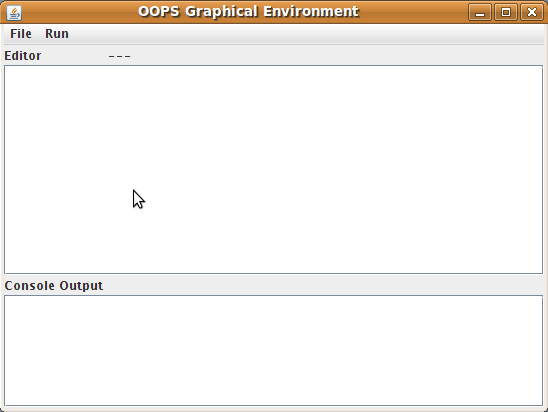
\includegraphics[width=0.7\textwidth]{demo01}
\end{frame}

\begin{frame}
\frametitle{Demonstration}
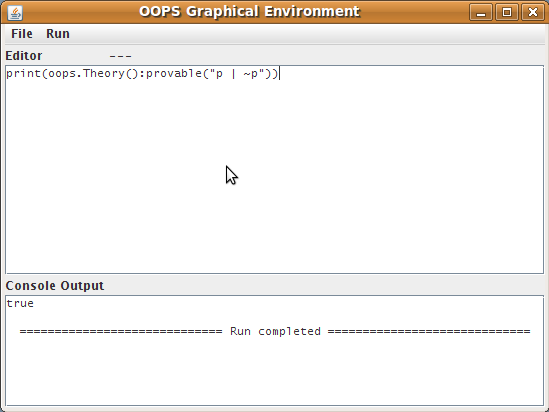
\includegraphics[width=0.7\textwidth]{demo02}
\end{frame}

\begin{frame}
\frametitle{Demonstration}
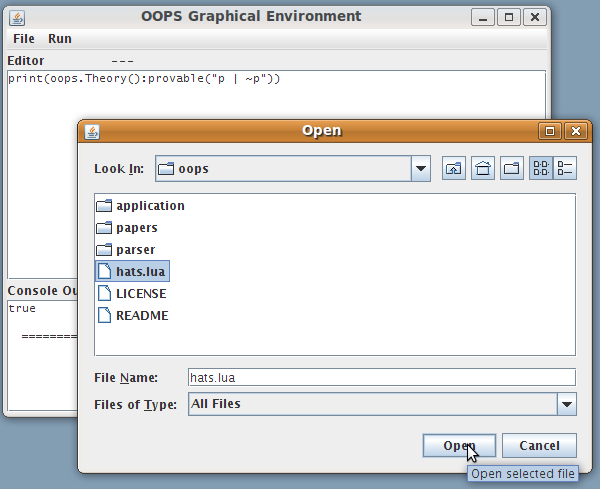
\includegraphics[width=0.7\textwidth]{demo03}
\end{frame}

\begin{frame}
\frametitle{The Puzzle (part 1)}
Initial situation:
\begin{itemize}
\item There are two wise persons: Abelard (1) and Heloise (2)
\item There are 3 hats, two red (r) and one white (w)
\item Each wise person wears a hat
\item Each wise person can see the other's hat
\item Each wise person can {\em not} see his/her own hat
\end{itemize}
Can they figure out their own hat's color?
\end{frame}

\begin{frame}[fragile]
\frametitle{Model: initial situation}

\begin{lstlisting}
-- agents[1] = "Abelard", agents[2] = "Heloise"
agents = {"Abelard", "Heloise"}

-- propositions:
-- r1: Abelard wears a red hat
-- w1: Abelard wears the white hat
-- r2: Heloise wears a red hat
-- w2: Heloise wears the white hat
\end{lstlisting}

\end{frame}

\begin{frame}[fragile]
\frametitle{Model: initial situation}
\begin{lstlisting}
-- each person has only one hat
oneHat = "(r1 = ~w1) & (r2 = ~w2)"
\end{lstlisting}
\pause
\begin{lstlisting}
-- there is only one white hat
oneWhite = "(w1 > r2) & (w2 > r1)"
\end{lstlisting}
\pause
\begin{lstlisting}
-- Abelard can see Heloise's hat
abelardSees = "#_1 w2 | #_1 r2"
\end{lstlisting}
\pause
\begin{lstlisting}
-- Heloise can see Abelard's hat
heloiseSees = "#_2 w1 | #_2 r1"
\end{lstlisting}
\end{frame}

\begin{frame}[fragile]
\frametitle{Model: initial situation}
\begin{lstlisting}
-- background knowledge:
background = conj(conj(oneHat, oneWhite),
    conj(abelardSees, heloiseSees))

-- add the background and the wise persons'
-- knowledge about it (to depth 2)
th = oops.Theory()
th:add(background)
th:add(knows("1", background))
th:add(knows("2", background))
th:add(knows2("2", "1", background))
th:add(knows2("1", "2", background))
\end{lstlisting}
\end{frame}

\begin{frame}[fragile]
\frametitle{Model: initial situation}
\begin{lstlisting}
-- print knowledge state of agent
function printKnowledge(th, agent)
    -- ... 
end

-- print knowledge state of Abelard
function printAbelard(th)
    printKnowledge(th, 1)
end

-- print knowledge state of Heloise
function printHeloise(th)
    printKnowledge(th, 2)
end
\end{lstlisting}
\end{frame}

\begin{frame}[fragile]
\frametitle{Model: initial situation}
\begin{lstlisting}
-- make sure we can show the counter model
oops.attachModelConstructor()

print("Initial Situation: ")
printAbelard(th)
printHeloise(th)
\end{lstlisting}
\begin{block}{Output}
\verb!Initial Situation:! \\
\verb!Abelard doesn't know! \\
\verb!Heloise doesn't know!
\end{block}
\end{frame}

\begin{frame}[fragile]
\frametitle{Model: initial situation}
\begin{lstlisting}
oops.showModel()
\end{lstlisting}
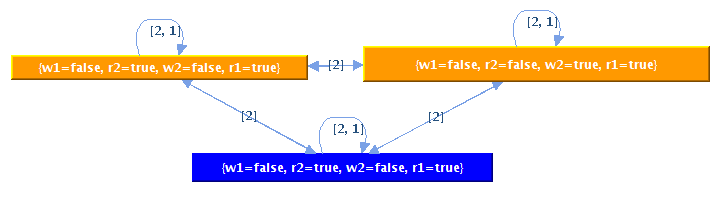
\includegraphics[width=\textwidth]{demo04}
\end{frame}

\begin{frame}
\frametitle{The Puzzle (part 2)}
\begin{itemize}
\item Abelard is asked if he knows the color of his hat
\item Abelard announces that he doesn't
\item Now Heloise knows the color of her hat
\end{itemize}
What is the color of Heloise's hat?
\end{frame}

\begin{frame}[fragile]
\frametitle{Model: after Abelard's announcement}
\begin{lstlisting}
-- After Abelard announces he doesn't know:
abelardKnows = "#_1 w1 | #_1 r1"
th:add(oops.Formula("#_2 ~ F"):substitute(
    {F = abelardKnows}, {}))
\end{lstlisting}
\end{frame}

\begin{frame}[fragile]
\frametitle{Model: after Abelard's announcement}
\begin{lstlisting}
print()
print("After Abelard's announcement: ")
printAbelard(th)
oops.showModel()
printHeloise(th)
print("Consistent: " .. tostring(th:consistent()))
\end{lstlisting}
\end{frame}

\begin{frame}[fragile]
\frametitle{Model: after Abelard's announcement}
\begin{block}{Output}
\verb!After Abelard's announcement:! \\
\verb!Abelard doesn't know! \\
\verb!Heloise knows his/her hat is red! \\
\verb!Consistent: true!
\end{block}
\end{frame}

\begin{frame}
\frametitle{Model: after Abelard's announcement}
Abelard still doesn't know:
\only<1>{
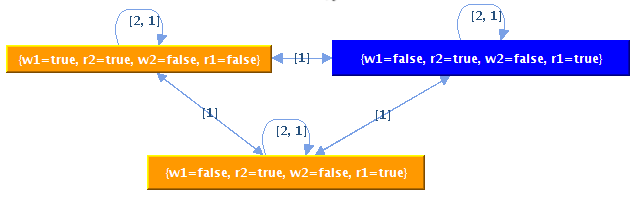
\includegraphics[width=\textwidth]{demo05}
}
\only<2>{
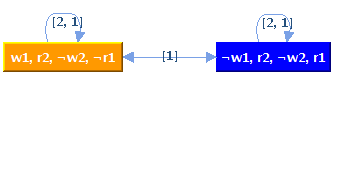
\includegraphics[width=\textwidth]{demo06}
}
\end{frame}

\section{Conclusion}
\subsection{}

\begin{frame}
\frametitle{Conclusion}
{\tt OOPS} has some interesting features:
\begin{itemize}
\item Cross-platform, easy to run, open source
\item GUI and integrated scripting
\item Tableau visualization
	\begin{itemize}
	\item Sometimes useful when `debugging' simple models
	\item Useful when learning tableau methods (check your own answers)
	\end{itemize}
\item Counter model visualization
	\begin{itemize}
	\item Useful when learning about Kripke semantics
	\item Useful when `debugging' less simple models
	\end{itemize}
\end{itemize}
\end{frame}

\begin{frame}
\frametitle{Future Work}
However, much remains to be done:
\begin{itemize}
\item Provide nicer Lua interface (implemented in Lua)
\item Be able to specify proof rules in Lua
\item More efficient proof algorithm
\item Formula simplification
\item Kripke models:
	\begin{itemize}
	\item Construct / alter models through scripting
	\item Model checking
	\item Bisimulation
	\end{itemize}
\item {\tt OOPS} as a Lua library (in addition to vice versa)
\end{itemize}
\end{frame}

\end{document}
